%preamble
% \documentclass{article}
\documentclass[journal]{IEEEtran}

%sets length of spacing between paragraphs
% \setlength{\parskip}{1em}

\usepackage{hyperref}

\usepackage{graphicx}
\graphicspath{ {images/} }

\synctex=1

\usepackage{lipsum}
\usepackage{pgf-pie}
\usepackage{adjustbox}
\usepackage{float}
%title page
\title{Mass Effect 3 and the ????? Racism or Tensions Between Alien Species\\
\vspace{.25cm}\large ENGL 199 Research Report \vspace{-.5cm}}
\author{\LARGE Arun Woosaree}
\date{\today}
%actual document
\begin{document}
\maketitle %insert titlepage here

\begin{abstract}
 Video games are often blamed for many social problems, from laziness and lack of motivation to accomplish anything, to pent up aggression that gets released as acts of violence in the real world. Although the gameplay in the Mass Effect Series contains violence, by allowing the player to develop his/her own character, the narrative of the game causes players to think about societal issues that we have problems with today, and act as a leader for the galaxy.
\end{abstract}

\LaTeX{} IEEE style:
%ieee style help:
\url{https://www.overleaf.com/15366912ngxtshbtbmhm#/58219789/}
%Introduction
\section{Introduction}
\textit{This introduction is far from complete, and only has ideas jotted down}
\\ \\
\textbf{Conflicts to talk about:}
\begin{itemize}
 \item Krogans and Salarians - Genophage
 \item working with the council against Cerberus. Cerberus is basically a pro human hate group analagous to white supremists today
 \item Quarians and geth - is synthetic life important?
\end{itemize}
-reapers- exterminate all organic life in a cycle every 50,000 years
\\ \\
\textbf{Statistics:}
\begin{enumerate}
 \item 92\% of players cured the genophage
 \item 64.5\% chose the paragon(good) options and 35.5\% the more mean shepard - can be the `no' part of the qualified argument for paragraph 1
 \item 27\% choose to save the quarians, 37\% the geth, and 36\% both
\end{enumerate}
-over 88.3 hours played in single player campaign
\\ \\
\textbf{Outline:}
\begin{itemize}
 \item Introduction:
       \begin{itemize}
        \item general statement ( importance of the topic)
        \item thesis sentence (opinons and why, make a qualified argument)
       \end{itemize}
 \item Body paragraphs: Start with the concession , then continue with arguments supporting your opinion
       \begin{enumerate}
        \item No
        \item Yes
        \item Yes
       \end{enumerate}

\end{itemize}
...with over 88.3 million hours spent by players in the single player campaign.\cite{ea}...
Although video games are commonly blamed for aggression in society today,
and the desensitising of indivisuals with respect to serious societal issues, Mass Effect  touches on some very important societal issues today, and
makes the player think about political views. One of the prevalent issues in the world today is
racism. Particularly, In the Mass Effect 3, the issue of racism is portrayed through alien characters, and
tensions between them, where the player makes decisions literally as a world leader. The game puts the player in the position to
make important decisions, which impact the outcome at the end of the game, and good decisions are rewarded.

The narrative takes place in the future, where humans are no longer concerned about racism amonsgt themselves but rather societal
tensions are between alien races. (If anything there are ideological tensions ie. with cerberus and the alliance but these
tensions are not a result of racism amonsgt humans, but rather different ideological views of what is the best interest for the human race. (cerberus believes in using any methods (even illegal and terrorist like) for furthuring the human race.)
both organizations goals are to ultimately do what they believe is best for the entire human race). Rather, racial tensions are observed betweeen different alien races.

\begin{figure}
 
\includegraphics[scale=2]{paragon}
 \caption{Most players choose on their own accord to be a kind leader as opposed to a ruthless one who gets the job done. \cite{ea}}
\end{figure}
%Talking about the Environment
%\newpage

\section{Human conflict - Cerberus Terrorist organization}
The allied aliens work together in a sort of galactic united nations-like government comprised of the most powerful sentient species, called the Council. Citadel. Cerberus throws in a monkey wrench and claim to be pro human,
but in reality are extremists who even illegally experiment on humans,
and ruthlessly kill those who do not agree with their ideology

-Renegade and paragon statistic most people chose to be a good leader as opposed to a ruthless one.
``Cerberus is a human-survivalist paramilitary group led by the enigmatic Illusive Man. Cerberus' core belief is that humans deserve a greater role in the galactic community, and that the Systems Alliance is too hamstrung by law and public opinion to stand up effectively to the other Citadel races. Cerberus supports the principle that any methods of advancing humanity's ascension are entirely justified, including illegal or dangerous experimentation, terrorist activities, sabotage and assassination. Cerberus operatives accept that these methods are brutal, but believe history will vindicate them. Nevertheless, both the Systems Alliance and the Citadel Council have declared Cerberus to be a terrorist organization and will prosecute identified Cerberus agents accordingly. ''\cite{wikia}

The player's goal is to unite the aliens against the reapers, as
previous civilizations have failed due to one species dominating the others.


``The greatest threat in the game then is not so much the Reapers, but the xenophobic prohuman faction called Cerberus who seek to use Reaper technology to impose human dominance over the galaxy. The explicitly racist undertones of Cereberus’ spokesman, the Illusive Man (voiced by Martin Sheen), contrasts Shepard’s multiculturalist project.''\cite{chrisb}
% \lipsum[3-4]


%Reason 2
\section{Tensions Between The Krogan and the Salarians}
these alien races distrust each other because one developed a virus to wipe the
other out. A staggering 92\% of the players choose to cure the genophage, which
eases diplomatic tensions, and is considered the good option. -and also,
only 3.8\% shot Mordin, a
% \lipsum[1-2]
\adjustbox{margin=10}{}
\begin{figure}
 \begin{adjustbox}{width=.4\textwidth}
  
\begin{tikzpicture}
   \pie[pos={8,8},radius=1,explode =0.15]  {92/Cured, 8/Not Cured}
  \end{tikzpicture}
 \end{adjustbox}
 \caption{Most players chose to cure the genophage \cite{ea}, an important diplomatic step for gaining military support of the Krogan, to the disappointment of the Salarians.}
\end{figure}
which is generally considered the ``good'' thing to do, since the Krogan have suffered due to this disease brought on them by the Salarians.


%Reason 3
\section{Are A.I. as important as Organic Life?}
The Quarians, who developed machines called the geth to do work made these
machines more advanced, and in violation of the Citadel's rules these machines
become a fully blown self-aware Artificial intelligence. The Quarians attempt to wipe them out, but the geth retaliate, and the Quarians lose millions of people, and are now nomads, and lose representation on the Citadel.
The player chooses between saving the Quarians, or gaining the military support of the geth, who have free will.

Ultimately, at the end of the game, the player chooses between destorying
all synthetic life, taking control of it, or merging organic and synthetic life,
thus reaching the ``pinnacle of evolution''\cite{me}
% \lipsum[5-6]
\adjustbox{margin=10}{}
\begin{figure}
 \begin{adjustbox}{width=.35\textwidth}
  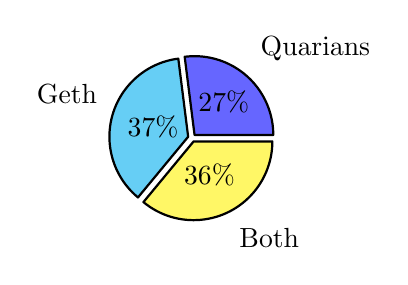
\begin{tikzpicture}
   \pie[pos={8,8},radius=1,explode =0.05]  {27/Quarians, 37/Geth, 36/Both}
  \end{tikzpicture}
 \end{adjustbox}
 \caption{Players appear to place as much value in synthetic life as in organic life. \cite{ea}}
\end{figure}

%Conclusion
\section{Conclusion}
\lipsum[7]
%causes all references in the bib file to be cited, even though you don't mention them in the paper
\nocite{*}
\bibliographystyle{IEEEtran}
\bibliography{references}

\begin{figure}[]
 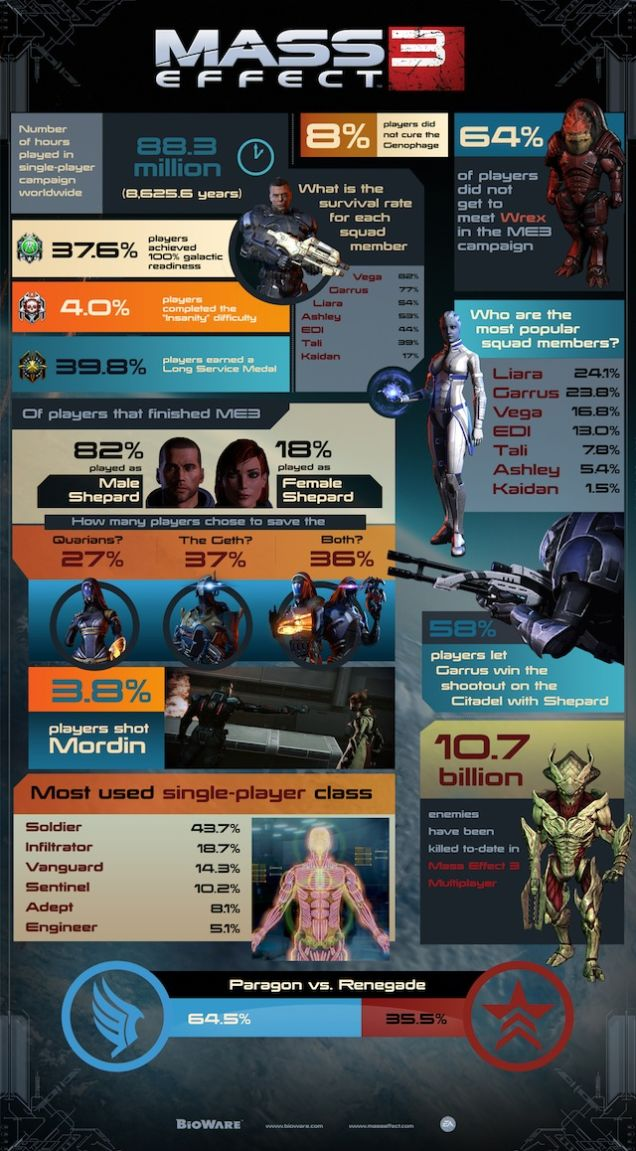
\includegraphics[width=.45\textwidth]{stat.jpg}
 \caption{Additional statistics. \cite{ea}}
\end{figure}
\end{document}
